\documentclass[final]{beamer}
\usetheme{SD}
\usepackage[orientation=landscape,size=custom,width=160,height=90,scale=1.9,debug]{beamerposter}
%\usepackage[absolute,overlay]{textpos}
%\setlength{\TPHorizModule}{1cm}
%\setlength{\TPVertModule}{1cm}

\title{BioConductor:  Open Source Tools for the Analysis and Comprehension of the Transcriptome}
\author{Bioconductor Core Development Group}
\footer{More information at \texttt{\url{http://bioconductor.org/}}}
\date{January 13, 2015}

\begin{document}
\begin{frame}[t]
  \begin{columns}[t]
    \begin{column}{0.24\linewidth}
      \begin{block}{What is Bioconductor?}
        Bioconductor provides tools for the analysis and comprehension of high-throughput genomic data.
        \begin{itemize}
        \item{Open source and totally free}
        \item{Collection of 1295 software packages}
        \item{Active user (100k downloads/year) and developer (>4000 contributors) communities}
        \item{Cloud-scale with Amazon Machine and Docker Images}
        \end{itemize}
      \end{block}
      \begin{block}{Genomic Data Analysis}
        \begin{itemize}
        \item{Microarray quality assessment and normalization}
        \item{RNA-seq, including single-cell quality control and normalization}
        \item{Exploratory data analysis}
        \item{Workflows available for:}
     \begin{itemize}
       \item{Gene expression}
       \item{Pathway analysis}
       \item{Alternative splicing and isoforms}
       \item{Fusion gene detection}
       \item{Variant calling and functional prediction}
     \end{itemize}
        \end{itemize}
      \end{block}
      \begin{block}{Functional Assays and Analysis}
        \begin{itemize}
        \item{CRISPR design, cleavage monitoring, and analysis}
        \item{Network reconstruction and gene regulation modeling}
        \item{Generic toolsets for analysis of niche sequencing approaches}
        \item{Flow cytometry tooling}
        \item{Image analysis for high content screening analysis}
        \end{itemize}
      \end{block}
      \begin{block}{Available Data Resources}
        \begin{itemize}
          \item{Microarray probe, gene, pathway, gene ontology, homology and other annotations} 
          \item{Online database access to Gene Ontology, KEGG, NCBI, Biomart/Ensembl, UCSC, and many other sources}
          \item{Experimental data packages including all of TCGA, Pharmacogenomics datsets, LINCS, and 400+ others}
        \end{itemize}
      \end{block}
    \end{column}
    \begin{column}{0.48\linewidth}
      \begin{block}{Graphical Capabilities of Bioconductor}
        \begin{columns}[t]
          \begin{column}{0.33\linewidth}
            \begin{figure}
              \centering
              \includegraphics[width=0.85\linewidth]{cir}
              \caption{A circos-like plot from the ggbio package}
            \end{figure}
            \begin{figure}
              \centering
              \includegraphics[width=0.85\linewidth]{interval}
              \caption{RNA-seq differential isoform expression from the ggbio package}
            \end{figure}
            \begin{figure}
              \centering
              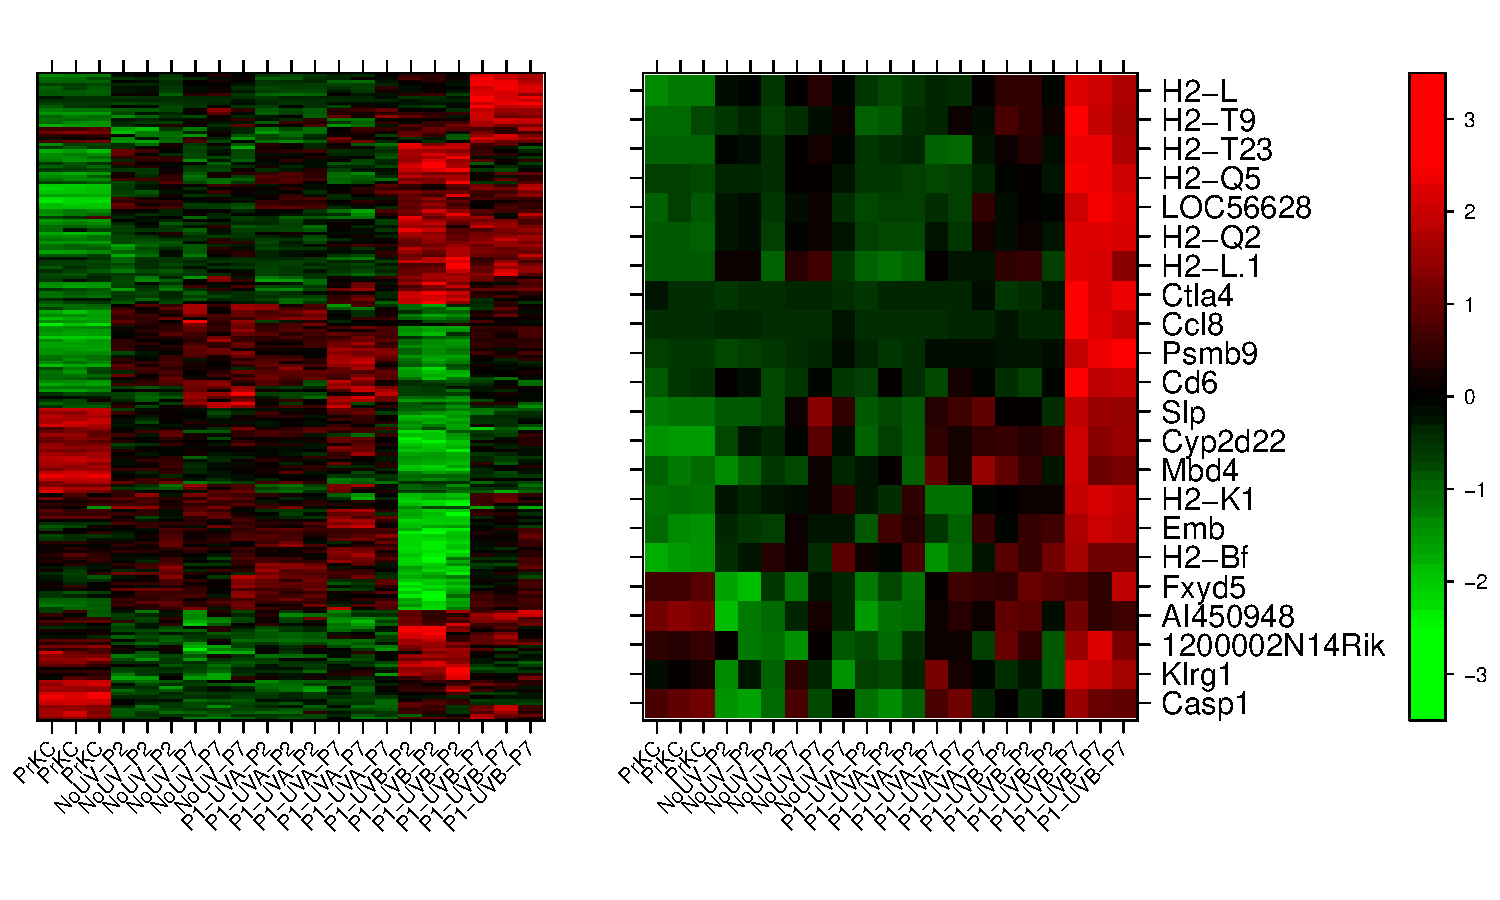
\includegraphics[width=0.85\linewidth]{heatmapPanels}
              \caption{Publication-quality graphics with R}
            \end{figure}
          \end{column}
          \begin{column}{0.33\linewidth}
            \begin{figure}
              \centering
              \includegraphics[width=0.85\linewidth]{flowFilter}
              \caption{Flow cytometry filtering and quantification}
            \end{figure}
            \begin{figure}
              \centering
              \includegraphics[width=0.85\linewidth]{stacked-darn}
              \caption{Genome overview plot from the ggbio package}
            \end{figure}
            \begin{figure}
              \centering
              \includegraphics[width=0.85\linewidth]{ebimage}
              \caption{Image segmentation using the EBImage package}
            \end{figure}
          \end{column}
          \begin{column}{0.33\linewidth}
            \begin{figure}
              \centering
              \includegraphics[width=0.85\linewidth]{rgraphviz}
              \caption{Arbitrary graph layout with Rgraphviz}
            \end{figure}
            \begin{figure}
              \centering
              \includegraphics[width=0.85\linewidth]{cosmo}
              \caption{Motif discovery and display with the cosmo package}
            \end{figure}
            \begin{figure}
              \centering
              \includegraphics[width=0.85\linewidth]{genomegraphs}
              \caption{Layer data and Ensembl annotation onto figures using GenomeGraphs}
            \end{figure}
          \end{column}
        \end{columns}
      \end{block}

 \end{column}
    \begin{column}{0.24\linewidth}
      \begin{block}{PrinciplesDesign, and Implementation}
        \begin{itemize}
        \item{Open source, open, community-driven development}
        \item{Reproducible research through strict versioning and literate programming approaches}
        \item{Statistical rigor}
        \item{Interoperability through purpose-built, rich data structures}
        \end{itemize}
      \end{block}
      \begin{block}{Design and Implementation}
        \begin{itemize}
        \item{Built using the R statistical programming environment}
        \item{Central infrastructure for code repository and continuous integration and builds}
        \item{NIH grant funded (NHGRI, NCI)}
        \item{Comprised of software packages, annotation packages, and experimental data packages}
        \end{itemize}
      \end{block}
      \begin{block}{Data Integration}
        Use of consistent data structures in the R statistical computing environment allows for complex data integration and multi-assay hypothesis generation and testing.
      \end{block}
      \begin{block}{Community, Training, and Education}
\small{Bioconductor runs training and education programs regularly throughout the year all over the world.  The annual Bioconductor Conference is held in Seattle each summer.  The Bioconductor support site is an interactive and online forum for discussion of Bioconductor software as well as statistical and informatics questions. Extensive online training materials are at the Bioconductor website.}
      \end{block}
      \begin{block}{Bioconductor Core Members}
        \small{Sean Davis (NCI), Vince Carey (Harvard), Wolfgang Huber (EMBL), Rafael Irizarry (Harvard), Levi Waldron (CUNY), Aedin Culhane (Harvard), Michael Lawrence (Genentech), Robert Gentleman (23andMe), and Martin Morgan (Roswell Park C.I.)}
      \end{block}
    \end{column}
    \end{columns}
  \end{frame}
\end{document}
